\listfiles
\documentclass[review]{elsarticle}

\usepackage[usenames]{color}
\usepackage{lineno,hyperref}
\modulolinenumbers[5]


\usepackage{graphicx} %package to manage images
\graphicspath{ {./images/} }


\usepackage{multicol}
\usepackage[ruled]{algorithm2e}\usepackage{booktabs}
\usepackage[ruled]{algorithm2e}
\SetKwComment{Comment}{$\triangleright$}{}
\usepackage{inputenc}

%\journal{Journal of \LaTeX\ Templates}
%\bibliographystyle{elsarticle-num}
\bibliographystyle{abbrvnat}
\setcitestyle{authoryear}

\begin{document}

\begin{frontmatter}

\title{Afinaci\'on y an\'alisis de par\'ametros de algoritmos heur\'isticos para un problema de ruteo, mediante t\'ecnicas de simulaci\'on y m\'etricas estad\'isticas \tnoteref{mytitlenote}}


%% Group authors per affiliation:
\author{Julio César Garc\'ia Garc\'ia\fnref{myfootnote}}
\address{Monterrey, M\'exico}

%% or include affiliations in footnotes:
\author[mymainaddress]{Posgrado en Ingeniería de Sistemas, Universidad Aut\'onoma de Nuevo Le\'on, M\'exico \corref{mycorrespondingauthor}}

\cortext[mycorrespondingauthor]{Corresponding author}
\ead{jcgg.8805@gmail.com}


\begin{abstract}
Este reporte contiene la aplicación de métodos de simuación para la calibración de parametros de alta relevancia en el uso de metaheurísticas. Al representar la culminación del curso de Simulación se hace uso de algunos elementos (prácticas) vistos en clase. Este trabajo consta de una implementación en python de una heurística para resolver un problema de ruteo propuesto en el trabajo del Dr. \cite{angelbello2013}. Se propone la aplicación de métodos de simulación para la calibración de parámetros que afectan el desempeño de la heurística y finalmente se realiza un analísis estadístico adecuado.
\end{abstract}

\begin{keyword}
Calibración de Parámetros\sep Simulación. 
\end{keyword}

\end{frontmatter}

\linenumbers

%\begin{multicols}{2}

\section{Introducci\'on}

En la realidad, encontrar una soluci\'on exacta en algunos problemas no es computacionalmente alcanzable. Existen procesos dentro de la cadena de suministro que necesitan de buenas soluciones en un corto tiempo (segundos) para tomar una buena decisón, algunos casos t\'ipicos son: el ruteo de veh\'iculos, la programaci\'on de producci\'on, el manejo de inventarios, entre otros. Por lo anterior, surge la necesidad de desarrollar m\'etodos m\'as eficientes con el fin de encontrar la mejor soluci\'on posible en un tiempo de proceso considerable.

Algunos de los m\'etodos m\'as usados para este fin son los algoritmos heur\'isticos, el desempe\~no y costo computacional de este tipo de algoritmos normalmente est\'a relacionado con la definici\'on del valor adecuado de los par\'ametros que se utilizan en su estructura. En los problemas reales, siempre se sugiere que par\'ametros usar en base a la instancia (estructura del problema) que se desea resolver. 

En este trabajo se estudia la calibraci\'on de los valores de los par\'ametros antes mencionados  as\'i como el desempe\~no y costo computacional del algoritmo acorde a dicha calibraci\'on, haciendo uso de simulaci\'on y de un adecuado an\'lisis estad\'istico.

\section{Planteamiento del Problema}

En la mayor\'ia de los problemas de optimizaci\'on surge la necesidad de desarrollar algoritmos de soluci\'on con el fin de aprovechar la estructura del problema a resolver y obtener soluciones de calidad aceptable en un tiempo computacional aceptable. 

A lo largo de la estructura de los algoritmos heur\'isticos, la mayor\'ia de las veces, se implementan algunos par\'ametros para la selecci\'on de candidatos, evaluaci\'on de objetos/objetivos y toma de decisiones en general. El desempe\~no que alcance un algoritmo en su implementaci\'on depende en gran medida de estos par\'ametros.

Dada la importancia de los par\'ametros del algoritmo, el problema secundario que se debe resolver para el uso eficiente del algoritmo consiste en lo siguiente: Calibrar adecuadamente los valores de los par\'ametros para que el heur\'istico en cuesti\'on sea lo m\'as robusto posible y tenga un buen desempe\~no (costo computacionalmente bajo y soluciones de buena calidad).

Se plantea el uso de experimentaci\'on y an\'alisis estad\'istico de los resultados obtenidos, lo anterior con el fin de obtener valores adecuados para los par\'ametros participantes y que reflejen un buen desempe\~no generalizado en el comportamiento del algoritmo. Se busca con esto una combinaci\'on de valores de par\'ametros que en la gran mayor\'ia de los casos ayuden al algoritmo a alcanzar soluciones de excelente calidad, m\'as a\'un,  se podr\'ia definir para cada instancia particular la combinaci\'on de los valores de par\'ametros que optimizan el desempe\~no del algoritmo en la misma.

\section{Antecedentes}

La calibración de parámetros es altamente relevante por su importancia para el performance de los algoritmos heurísticos por lo que en muchos trabajos se ha estudiado su efecto y su adecuada calibración, por ejemplo:

\begin{itemize}
\item Algoritmos evolutivos (ver \cite{afinacionEvolutivo}).
\item Algoritmos bio-inspirados, por ejemplo el algoritmo de enjambre de partículas (ver \cite{afinacionEnjambre}).
\item Algoritmos genéticos basados en lógica difusa (ver \cite{afinacionLogicaDifusa}).
\end{itemize}

Es evidente que la calibración de parámetros es un tema necesario, sobre todo en el PISIS por los algortimos que se desarrollan en este posgrado, esa importancia fue la detonante de la elección de este tema para trabajo final. 

\section{Metodolog\'ia de Soluci\'on}
Previo a la afinaci\'on de los par\'ametros, en este trabajo se presenta un algoritmo basado en GRASP para resolver un problema de ruteo. El problema de ruteo es planteado en el trabajo escrito por \cite{angelbello2013}, el cual consiste en encontrar una ruta en un grafo V donde cada nodo de la red representa un cliente y debe ser visitado una sola vez, el nodo donde inicia y termina la ruta es un nodo ficticio. El objetivo del problema consiste en minimizar la latencia total.

Enseguida se presenta el Pseudoc\'odigo  del algoritmo basado en la metaheur\'istica GRASP, el cuál, se rediseñó dicho algoritmo en base a la propuesta  del trabajo escrito por \cite{angelbello2013}.

Se definen los siguientes conjuntos: $ Clientes$, Lista Restringida de Candidatos ($LRC$) ,  Solución ($Sol$) y el Total de Iteraciones ($Iter$).


\begin{algorithm}[H]\footnotesize		
	$S^* \leftarrow S_c$ \;
    \For{$k \in Iter$}{	
        \While{$Clientes \not= \emptyset$}{
        	Para cada $i \in Clientes $  calculas la Latencia Parcial (LP) en el último punto de inserción\;
        	$LP_{min} \leftarrow$ min\{ $LP_i, tal que,  i \in Clientes $ \}\;	
        	$LP_{max} \leftarrow$ max\{ $LP_i, tal que,  i \in Clientes $ \}\;	
        	$LRC \leftarrow$ \{ $j \in Clientes, tal que, LP_j <= LP_{min} + \alpha (LP_{max} - LP_{min} )$\}\;	
        	Se \vspace{1mm}selecciona un elemento aleatorio $l  \in RCL$ y se inserta en la última posición de la $Sol$
        }
        \If{ Se \vspace{1mm} requiere Búsqueda Local  }{
    		 $S$= $B\acute{u}squeda$ \vspace{1mm} $Local$ \vspace{1mm} $Intercambio(S)$\;
    	}
    	\If{ $Latencia(S) \leq Latencia(S_{Best}) $  }{
            $S_{Best}=S$\;
        }
    }
\Return $S_{Best}$

	\label{algoritmo}
	\caption{Simulación basado en GRASP}	
\end{algorithm}

Para el algoritmo de Búsqueda Local Intercambio, se busca realizar intercambio en clientes consecutivos dentro de la ruta, siguiendo un orden consecutivo en la solución. Para la primer mejora, basta con que se realice el primer movimiento que mejore (minimize) la función objetivo actual de la ruta. Si se realiza la mejor mejora, se tendrá que realizar un ciclo para todos los clientes consecutivos de la ruta y por lo cuál, pueden existir diversos movimientos que mejoren la función objetivo de la ruta. 
	
 La implementación original de este algoritmo se realizó en el lenguaje de programación C++, debido a que surgió de un trabajo requerido para la aprobación de un curso también de la maestría. En este trabajo, la implementación de dicho algoritmo se migró a Python para realizar dicha simulación. La diferencia del algoritmo rediseñado en este trabajo comparado contra el original, consiste en que se cambió la función a evaluar ($LP$) tanto en la construcción de la solución como en el método de Búsqueda Local. Además, se optó por realizar la variantes en el algoritmo considerando sólo la primer mejora, la mejor mejora y omitirla, por lo cuál, se tienen dos variantes del trabajo original.

Los códigos correspondientes a este trabajo pueden ser encontrados en el repositorio https://github.com/Julio-Garcia-Garcia/Simulacion/tree/master/Proyecto (\cite{repositorio}).

\section{Experimentaci\'on y Resultados
}
Los par\'ametros analizar en este trabajo son el valor alpha ($\alpha$), el cual est\'a relacionado con la cantidad de elementos que participan en la lista restringida de candidatos  y la cantidad de iteraciones del algoritmo ($Iter$). Los valores de alpha son entre cero y uno con un paso definido de 0.1, mientras que los valores de iteraciones se consideran desde 1000 hasta 5000 con paso de 1000. 

Para este experimento se decidi\'o realizar 5 réplicas, las cuales se efectuar\'an con instrucciones de paralelismo ejecutadas desde Python, las m\'etricas (objetivos) a observar son las siguientes:

\begin{itemize}
\item F1: Funci\'on objetivo,latencia de todos los clientes
\item F2: Tiempo total de ejecuci\'on del algoritmo 
\end{itemize}

Como se comentó anteriormente, la experimentacion fue realizada con tres versiones de algoritmo, cada una de ellas corrida sobre tres instancias, estás  contienen 10, 20 y 50 clientes (nodos) respectivamente. Cada versión de las corridas, además, fue replicada sobre 1, 2 y 3 procesadores paralelizando las réplicas con la finalidad de reducir los tiempos de experimentación.

En la primer versión (A) se tiene el código original basado simplemente en el método constructivo de GRASP, sin la búsqueda local. El la segunda versión (B) se incluye, además, la implementación de una búsqueda local que se rompe cuando se encuentra la primer mejora inter-ruta. En la tercera y última verisón (C) se tiene la mencionada búsqueda local pero con la mejor de todas las mejoras. 

Cabe mencionar que los límites inferiores y superiores de los parámetros de cantidad de réplicas e iteraciones fueron propuestos en base al alto costo computacional que representa esta experimentación.

\subsection{Comparación de tiempos}

Dado que se tienen tres versiónes diferentes del algoritmo implementado y tres posibilidades de procesadores a utilizar (1, 2 o 3), surge la necesidad de comparar el tiempo computacional requerido para la experimentación.

La siguiente imagen muestra un diagrama de caja y bigotes en el que se grafican los tiempos computacionales utilizados a nivel cantidad de nodos - tipo de algoritmo, de tal forma que la leyenda "10\_B" significa que la instancia contiene 10 nodos y que la experimentación se hizo utilizando la versión B del algoritmo (algoritmo basado en GRASP + la implementación de una búsqueda local que se rompe cuando se encuentra la primer mejora inter-ruta).

	 \begin{figure}[h!]
	\centering
	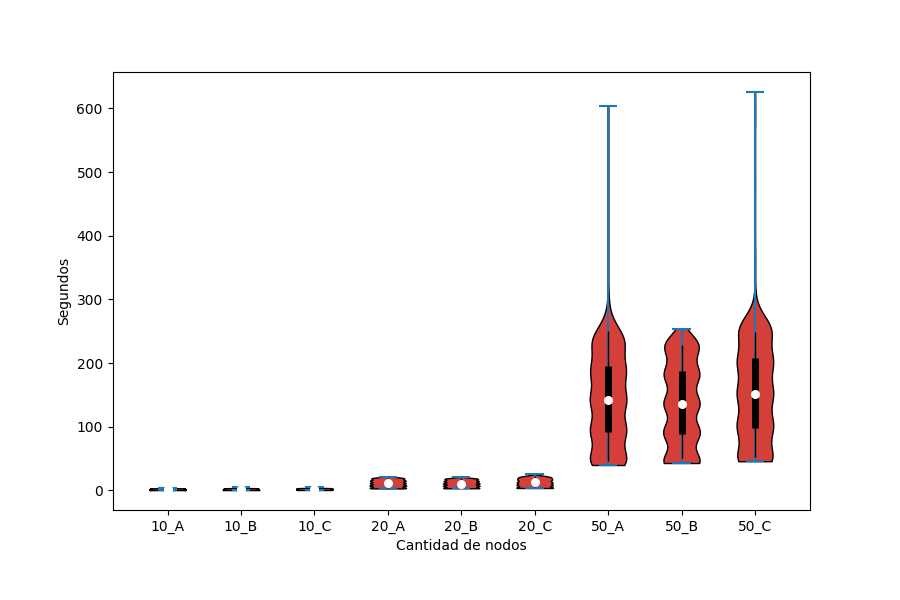
\includegraphics[width=0.7\linewidth]{tiempos.png}
	\caption{Tiempo computacional por cantidad de nodos - versión de algoritmo.}
	\label{fig:imagen1}
	%\newpage
	
	\end{figure}
%\includegraphics[width=\textwidth]{Tiempos}

Notoriamente, conforme se va aumentando la cantidad de nodos en la red, se aumenta también el tiempo computacional requerido. 

A continuación, se muestra el diagrama de caja y bigotes en el que se grafican los tiempos computacionales utilizados a nivel cantidad de nodos - tipo de algoritmo paralelizando con 3 procesadores, se omitió analisis de cuando se usa un par de procesadores porque el de 3 es mejor.


	 \begin{figure}[h!]
	\centering
	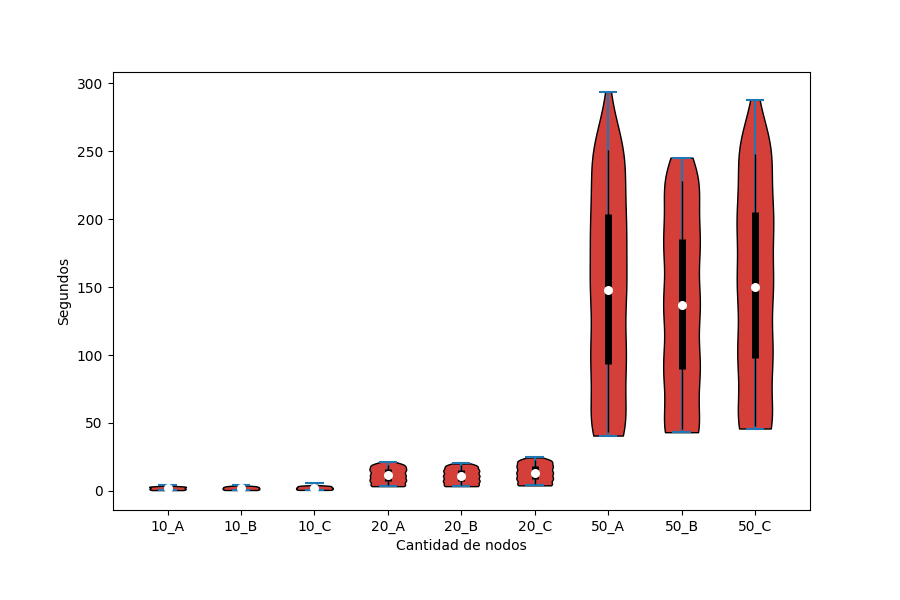
\includegraphics[width=0.7\linewidth]{3tiempos.png}
	\caption{Tiempo computacional por cantidad de nodos - versión de algoritmo paralelizando con 3 procesadores.}
	\label{fig:imagen2}
	%\newpage
	
	\end{figure}
%\includegraphics[width=\textwidth]{3Tiempos}

Se puede observar que el promedio del tiempo computacional utilizado es bastante parecido por corrida, sin embargo, se reducen notoriamente los puntos atípicos del diagrama y de manera natural se ahorra tiempo en la experimentación completa al poder correrse 3 réplicas al mismo tiempo. 

\subsection{Comparación de Latencia}

La siguiente imagen muestra un diagrama de caja y bigotes en el que se grafican los tiempos computacionales utilizados a nivel cantidad de nodos - tipo de algoritmo, de tal forma que la leyenda "10\_B" significa que la instancia contiene 10 nodos y que la experimentación se hizo utilizando la versión B del algoritmo (algoritmo basado en GRASP + la implementación de una búsqueda local que se rompe cuando se encuentra la primer mejora inter-ruta).

	 \begin{figure}[h!]
	\centering
	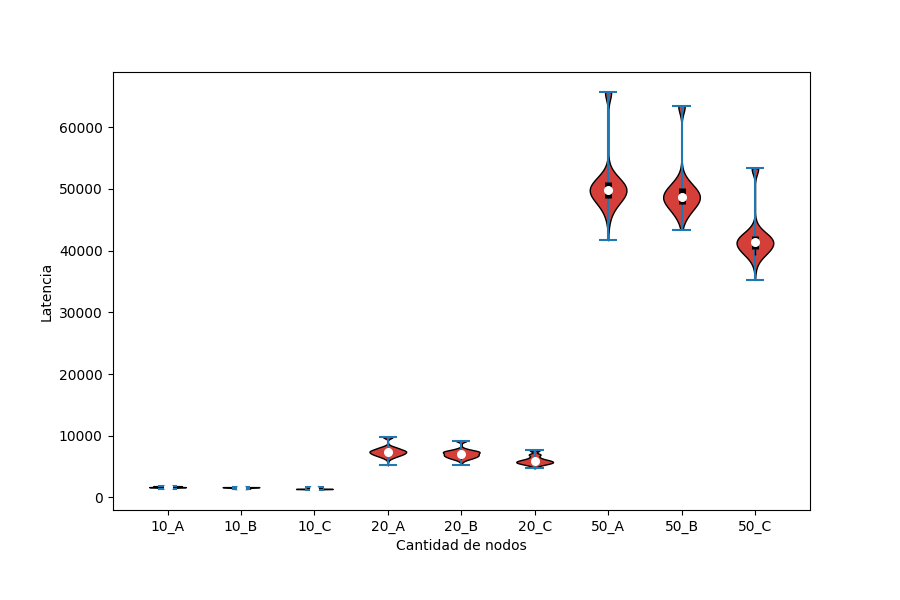
\includegraphics[width=0.7\linewidth]{latencia.png}
	\caption{Latencia por cantidad de nodos-versión de algoritmo.}
	\label{fig:imagen3}
	%\newpage
	
	\end{figure}
%\includegraphics[width=\textwidth]{Latencia}

Notoriamente, conforme va aumentando la cantidad de nodos en la red aumenta también la latencia que se obtiene en la mejor solución encontrada. 

A continuación, se muestra el diagrama de caja y bigotes en el que se grafica la función objetivo (latencia) alcanzada a nivel cantidad de nodos - tipo de algoritmo paralelizando con 3 procesadores, se omitió analisis de cuando se usa un par de procesadores porque el de 3 es mejor.

	 \begin{figure}[h!]
	\centering
	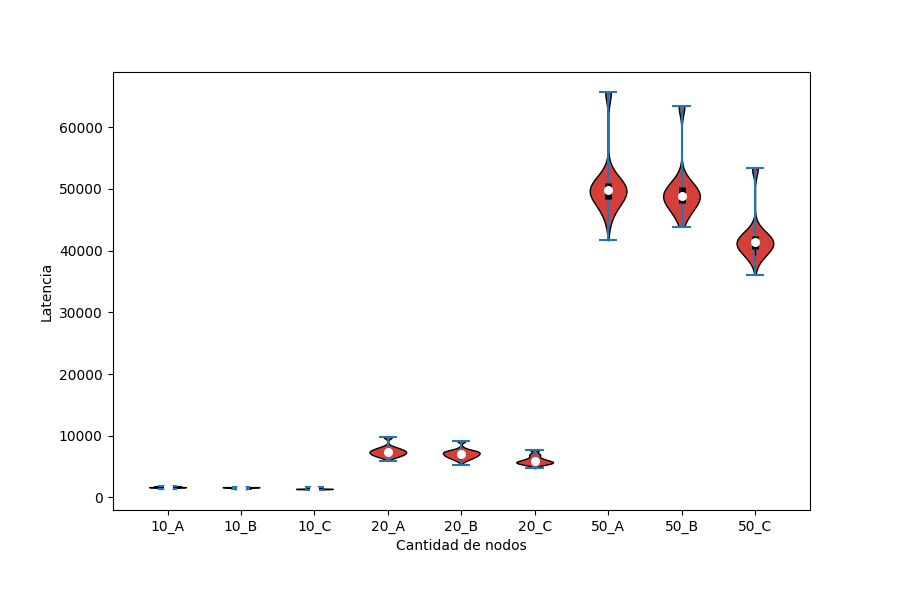
\includegraphics[width=0.7\linewidth]{3latencia.png}
	\caption{Latencia por cantidad de nodos - versión de algoritmo paralelizando con 3 procesadores.}
	\label{fig:imagen4}
	%\newpage
	
\end{figure}
%\includegraphics[width=\textwidth]{3Latencia}

Se puede observar que la calidad de las soluciones alcanzadas es bastante parecido al experimento total, sin embargo, se reducen notoriamente los puntos atípicos del diagrama. 

Con esta imagen, además, se puede hacer una comparación de la calidad de las soluciones obtenidas por las tres versiones del algoritmo. Como era de esperarse, el algoritmo sin ninguna mejora es superado en calidad (Latencia) de soluciones por la versión del Algoritmo (B), sin embargo, el mejor de los comportamientos se alcanza con el algoritmo que posee la búsueda que reliza un análisis exhaustivo de los cambios inter-ruta y se queda con el mejor de los mismos (Algoritmo C).

\subsection{Frente de pareto}

En la práctica, existen procesos en los cuales los usuarios pueden esperar un tiempo en horas para encontrar una solución, por ejemplo, una planeación agregada (mensual). Sin embargo, hay procesos que su espera debe ser corta, por ejemplo, la asignación de operadores en los transportes, es aquí donde la programación multiobjetivo cobra relevancia. En este trabajo, se busca medir los objetivos de latencia y tiempo computacional, por lo cuál, se realizó un frente de pareto para  identificar los mejores valores usados por estos parametros, esto para garantizar robustez en el algoritmo. 

Para la graficación de los frentes de pareto se tomó como base el código de la practica 11: frentes de Pareto de la Dra. Elisa (ver \cite{frentePareto}). Al identificar las soluciones del frente de Pareto se puede con ellas identificar los valores utilizados para obtener dicha solución.

A continuacion, se muestra el frente de Pareto obtenido con la experimentacion de instancia con 10 nodos utilizando la versión A del algoritmo (solamente GRASP) y 3 procesadores. Cada punto coloreado en verde representa una solución dominante y que por tanto forma parte del frente Pareto, las soluciones en negrita son soluciones dominadas. Para cada una de ellas podemos identificar el valor de $\alpha$ y el número de iteraciones ($Iter$) utilizado.

 \begin{figure}[h!]
	\centering
	\includegraphics[width=0.7\linewidth]{10_A_frente.png}
	\caption{Afinación de parámetros.}
	\label{fig:imagen4}
	%\newpage
	
\end{figure}

%\includegraphics[width=\textwidth]{images/10_A_frente.png}

La siguiente imagen muestra con un cuadro azul la solución que se alcanzó utilizando el menor tiempo computacional, que es notorio que tiene una latencia muy alta. Con el círculo ámbar se identifica la solución de menor latencia, que evidentemente no tiene el menor tiempo computacional utilizado. Si, por ejemplo, lo único que nos interesara fuera saber cuales valores de $\alpha$ y del número de iteraciones utilizado necesitamos para obtener la menor latencia posible en esta instancia, las podríamos obtener de la solción marcada en ámbar y nos diría que la mejor combinación de valores es: $\alpha = 1$ y la cantidad de iteraciones en 4000.

 \begin{figure}[h!]
	\centering
	\includegraphics[width=0.7\linewidth]{10_A_mejores.png}
	\caption{Afinación de parámetros.}
	\label{fig:imagen4}
	%\newpage
	
\end{figure}
%\includegraphics[width=\textwidth]{images/10_A_mejores.png}



\section{Conclusiones y Trabajo a Futuro}

En la realidad, la calibración de parámetros se vuelve fundamental para lograr un comportamiento esperado en cada una de las estructuras (instancias) que se tienen en los problemas. Si bien, siempre existirá una sugerencia generica para los parámetros de un algoritmo, es imposible, que los valores de los parámetros sean los mismos para todas las instancias. La calibración ayuda a tener un mejor funcionamiento en los objetivos planteados.
Dentro del alcance y contenido de este trabajo se tienen:	
\begin{itemize}
\item Implementación en Python de un algoritmo basado en GRASP
\item Implementación de un método de búsqueda local
\item Simulación para la variación de parámetros en el algortimo
\item Paralelización de replicas en el algoritmo
\item Análisis estadístico para evaluar los parámetros variados
\item Obtención de Frente de Pareto
\end{itemize}

Basados en el analísis estadístico podemos afirmar que es notoria la diferencia en el desempeño del algoritmo a lo largo de todas la diferentes combinaciones de los valores de los parámetros, por lo que es de vital importancia su correcta elección.  Es evidente también que la calibración de parámetros abordada representa un problema de optimización en si misma, por lo que su dificultad también representa un reto.

Como trabajo a futuro se propone realizar experimentación con mayor cantidad de núcleos (nodos), así como agregar un objetivo más al problema original. Además, se pretende adaptar el Algoritmo Genético que se desarrolló en la clase de Simulación para el problema de ruteo presentado en este trabajo. 
%\end{multicols}

\bibliography{Biblio}

\end{document}